\documentclass[UTF8]{ctexart}
\usepackage{bookmark}
\usepackage{geometry}
\usepackage{hyperref}
\geometry{a4paper,scale=0.8}
\usepackage{ctex}
\usepackage[style=caspervector,backend=biber,utf8]{biblatex}
\usepackage{booktabs}
\usepackage{array}
\usepackage{fancyhdr}
\pagestyle{fancy}
\fancyhf{}
\renewcommand\footrulewidth{1pt}
\lhead{\textit{王铠泽}}
\rhead{\textit{PB18020766}}
\chead{\href{mailto:volar@mail.ustc.edu.cn}{\textit{volar@mail.ustc.edu.cn}}}
\rfoot{\textit{中国科学技术大学}}
\lfoot{\today}
\usepackage{graphicx}
\usepackage{float}
\usepackage{subfigure}


\begin{document}

	\centering\textbf{\LARGE{计算物理A第十次作业}}
	
	
	\textit{王铠泽\qquad PB18020766}
	
		
	\section{作业题目}
	
	\begin{itemize}
		\item 研究有取向的布朗粒子(如纳米棒)的随机行走,计算取向的自关联函数:
		$$C(t)=\langle u_x(t)u_x(0)\rangle$$
		其中$u_x$为取向单位向量在$x$轴上的投影。
		
	\end{itemize}

	\section{实现方法和原理}
	
	\begin{itemize}
		\item 模型建立
		
		为了简单起见,我们考虑一个形状为椭圆的二维纳米棒的随机游走,并假设其长轴长度为$a$,短轴长度为$b$。以椭圆长轴为$x'$轴,椭圆短轴为$y'$轴,原点在质心的惯性系作为我们讨论的出发点,通过坐标变换可以得到原实验室系的坐标$x,y$ 。写出$Langevin$方程:
		$$\left\{
		\begin{array}{lcl}
			 \ddot{x'}=-\frac{1}{B_1}\dot{x'}+f_{x'}\\
			\ddot{y'}=-\frac{1}{B_2}\dot{y'}+f_{y'}\\
			\ddot{\theta}=-\frac{1}{C}\dot{\theta}+\tau
		\end{array} \right.$$
		在这个最简单的假设下,$x',y',\theta$之间是完全没有任何耦合的。因为$a>b$,可以认为$B_1<B_2$。本文再加上一条假设:$\theta$方向转动远远慢于平动,$C<<a\cdot B_1/B_2$。[1]
		
		最后通过坐标变换到实验室系:
		
			$$\left\{
		\begin{array}{lcl}
		dx=cos\theta dx'-sin\theta dy'\\
		dy=sin\theta dx'+cos\theta  dy'
	
		\end{array} \right.$$
		
				\begin{figure}[H]
				\centering  %图片全局居中
				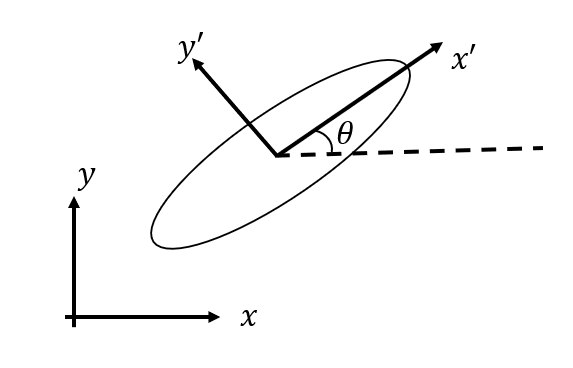
\includegraphics[width=3in]{1}
				\caption{模型示意图}
			\end{figure}
	


\begin{flushleft}
		由于三个方向解耦,可以算出各物理量二阶矩如下:
\end{flushleft}
	
	$$\langle x'^2 \rangle=2D_{x'}t$$
	$$\langle y'^2 \rangle=2D_{y'}t$$
	$$\langle \theta^2 \rangle=2D_\theta t$$
	\begin{flushleft}
		其中$D_{x'}=kTB_1,D_{y'}=kTB_2,D_\theta=kTC$
	\end{flushleft}

	这是由$x(t)$服从$N(x_0,\sqrt{2D_xt})$得到的。在下面的计算以及讨论中,为了方便起见,令$D_1,D_2,D_t$为三个解耦变量的正态分布的标准差。
	
	
	
	\item 理论结果
	
	对于自关联投影$C(t)$的计算:
	
	$\langle u(t)u(0) \rangle=\langle cos(\theta)cos(\theta_0) \rangle$,系综平均理解为对初始不同角度$\theta_0$和对大量随机运动的二重平均。而初始角度为$\theta_0$的纳米棒在$t$时间后角度的分布应该是$N(\theta_0,D^2_t t)$。
	
	$$\Rightarrow \langle cos(\theta)cos(\theta_0) \rangle=\int_{0}^{2\pi}d\theta_0\int_{-\infty}^{\infty}d\theta\frac{1}{\sqrt{2\pi {D_t} t}}cos(\theta) cos(\theta+\theta_0)exp[-\frac{\theta^2}{2D^2_t t}]=\frac{1}{2}exp(-\frac{D^2_t t}{2})$$
	
	在关于$x,y$的讨论上,虽然在$x'-y'$系中$x',y'$是可以视为互相独立的两个不同扩散系数的布朗运动,但由于要转换到实验室系中,出现了和角度之间的耦合,这时它们的分布就不再是简单的正态分布。一个较为定量化地描述和正态分布偏移的方法是计算位移的四阶累计量(cumulant)\cite{ref1}:
	$$C_{\theta_0}^{(4)}(t)=\langle [x(t)]^4 \rangle_{\theta_0}-3\langle [x(t)]^2 \rangle_{\theta_0}^2$$
	正态分布的四阶累积量为零。
	
	
	无量纲归一化后的指标是:
	
	$$p(t,\theta_0)=\frac{C_{\theta_0}^{(4)}(t)}{3\langle [x(t)]^2 \rangle_{\theta_0}^2}$$
	
	
	\item 计算实现方法
	
	\subitem 计算自关联函数
	
	进行两层循环:外层对系综进行循环(用$i$标记系统数),内层对时间进行循环(用$j$标记步长)。每次进行一个系统的循环时,初始化初始的夹角$\theta(0)=\theta_0$,为$[0,2\pi]$上的均匀分布。使用数组$T$来记录每一个时间下对应的$C(t)$的数值,并写入文件。
	
	\subitem 计算扩散系数$D_x,D_y$

	基本思路和计算自关联函数差不多,只是每对一个系统进行计算时,$\theta$不需要随机初始化,$\theta(0)=\equiv0$。注意对$x',y'$叠加时,每一步都是在原基础上叠加一个服从正态分布$N(0,D_{1/2}^2)$的长度。最后用数组$Dx,Dy$记录数据,并写入文件。
	
	\subitem 计算四阶累计量
	
	和上述思路差不多,仅是统计量换成$x^2,x^4$,进行记录。
	


	\end{itemize}

	\section{程式说明}
	
	
	\begin{itemize}
		\item rw1.c
		
		该程式计算在解耦情况下自相关函数$u(t)$的情况。
		
		\item rw2.c
		
		该程式计算在实验室系中扩散系数$D_x=\langle x^2(t) \rangle/t$和$D_x=\langle x^2(t) \rangle/t$的数据。
		
		\item cumulant.c
		
		该程式计算在该模型下的四阶统计量$C(t)$的数据。
		
		\item rdm.h
			
		这是一个包含了使用16807产生器生成指定长度的$[0,1]$上均匀分布随机数函数的头文件。
		
		\subitem void rdm(int N,double *x,int method)
		
		该函数将输入的指针$x$对应的长度为$N$的数组用$[0,1]$上的随机数填满。method是关于初始种子的选择。method=0:默认种子;method=1,时间种子。程式中故意采用$sleep$函数就是为了得到不同的时间种子。
		
		\item time\_seed.txt
		
		16807产生器抽样时对应的时间种子数据(每次1个种子)。调用多少次16807生成器就生成多少个数据记录。每一个分布对应的种子已经手动加上对应的实验了。种子产生公式如下:
		
		
		\begin{figure}[H]
			\centering  %图片全局居中
			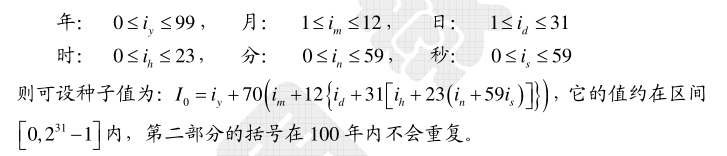
\includegraphics[width=4in]{2}
		\end{figure}
		
\textbf{		Tip:程序中多处使用了$sleep$函数是为了换时间种子,因而可能运行时间较久一点。}
	
		\item ensemble.txt
		
		这是取完系综平均的$D_x,D_y$数据文件,后面括号内为详细的实验条件。
		
		\item one\_ellipsoid.txt
		
		这是针对一个特殊的纳米棒的随机游走记录下其位移,转角随时间关系的数据文件,后面括号为详细的实验条件。
		
		\item cumulant.txt
		
		这是记录了四阶累计量数据的文件。
		
		
	\end{itemize}
	
	\section{计算结果}
	\begin{flushleft}
		选择正态分布的三个标准差分别为$D_1=1.0,D_2=0.01,D_t=0.05/0.08/0.10$做下面的计算并讨论。
	\end{flushleft}
	
	\subsection{单个纳米棒随机行走展示}
	
			\begin{figure}[H]
					\centering  %图片全局居中
					\subfigure[step=8]{
						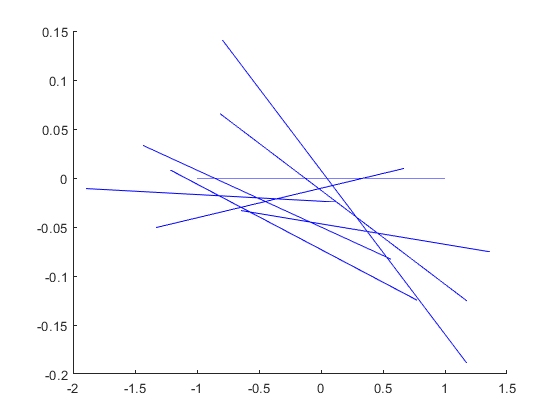
\includegraphics[width=0.45\textwidth]{8}}
				\subfigure[step=80]{
					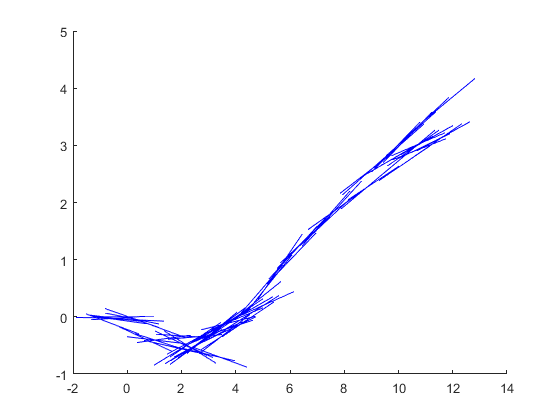
\includegraphics[width=0.45\textwidth]{80}}
						\subfigure[step=800]{
							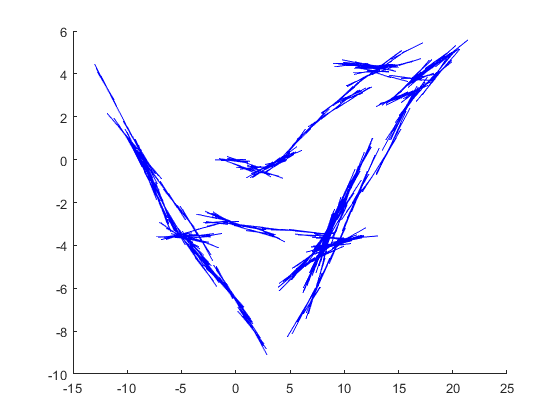
\includegraphics[width=0.45\textwidth]{800}}
							\subfigure[step=8000]{
								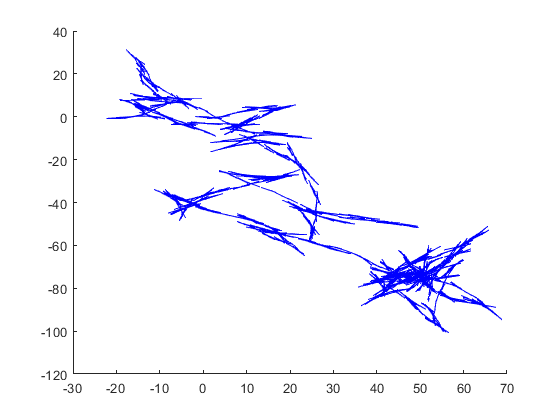
\includegraphics[width=0.45\textwidth]{8000}}
					\caption{纳米棒运动随着时间演化}
				\end{figure}
			
	\begin{flushleft}
		上面几个图将不同时间步长下的纳米棒运动形态做了一个展示,若将此过程进行下去,局部放大可以观察到自相似性。注意上图中纳米棒的形状简化为一根带取向(长轴方向)的直线。\textbf{\textit{更直观的运动演示请参见压缩包中的rw.gif文件(置于reslut文件夹下),记录了在前800步的纳米棒运动。}}
	\end{flushleft}
	
	\subsection{自关联函数计算}
	
	选取$D_t=0.5$,读入每一个时间步长对应的关联函数$c(t)$。用$Matlab$自带的拟合工具箱拟合结果如下:
	
	\begin{figure}[H]
		\centering  %图片全局居中
		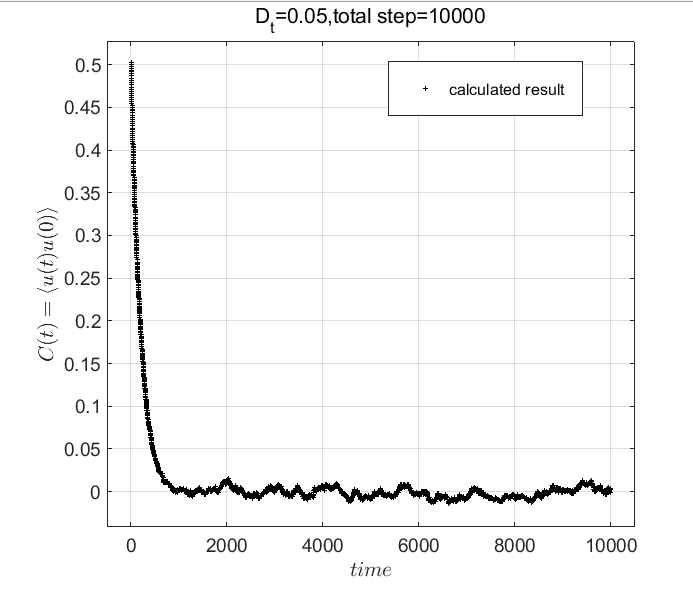
\includegraphics[width=4in]{3}
		\caption{实验数据}
	\end{figure}
	
\begin{flushleft}
		
	将下面的拟合结果和理论预言的$\frac{1}{2}exp(-\frac{D_t^2t}{2})$对比。可以发现非常接近理论语言,偏差的原因在于系综平均理想情况下应该是对无数多个系统平均,而此处仅取了10000个,会有毛刺状出现。
\end{flushleft}
	\begin{figure}[H]
		\centering  %图片全局居中
		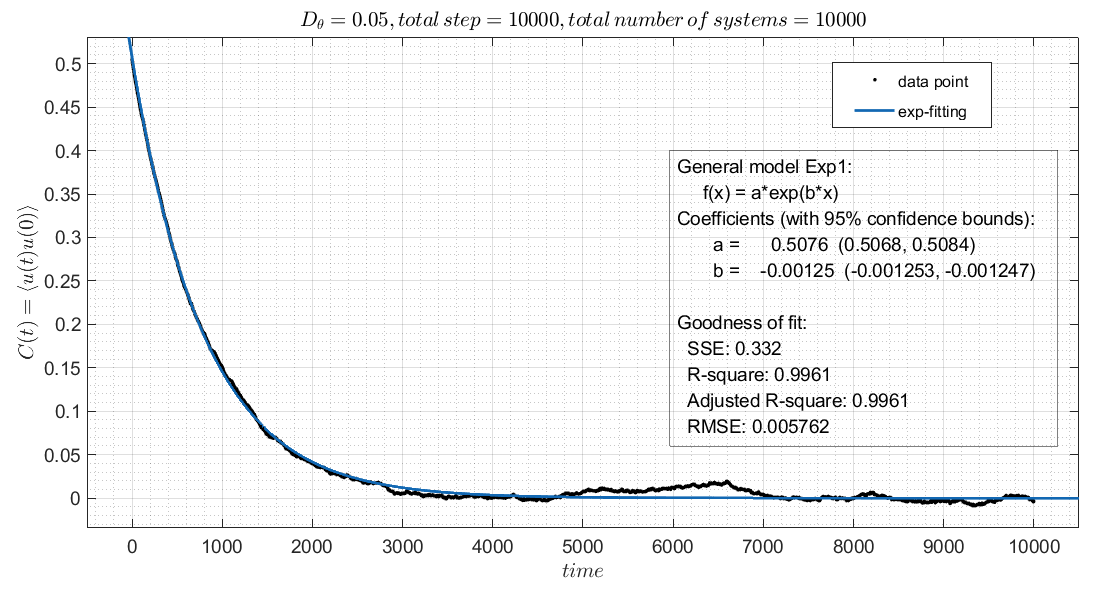
\includegraphics[width=6in]{rw}
		\caption{拟合结果}
	\end{figure}
	
	\newpage
	\subsection{扩散系数$D_x,D_y$计算}
	
	\begin{flushleft}
		下面给出在实验室系观察到的$D_x,D_y$的数值结果。通过$\langle x^2(y^2)\rangle/t$来计算这两个物理量。调整不同的$D_t$,即$\theta$方向的转动速度来观察变化。
	\end{flushleft}
	
	\begin{figure}[H]
		\centering  %图片全局居中
		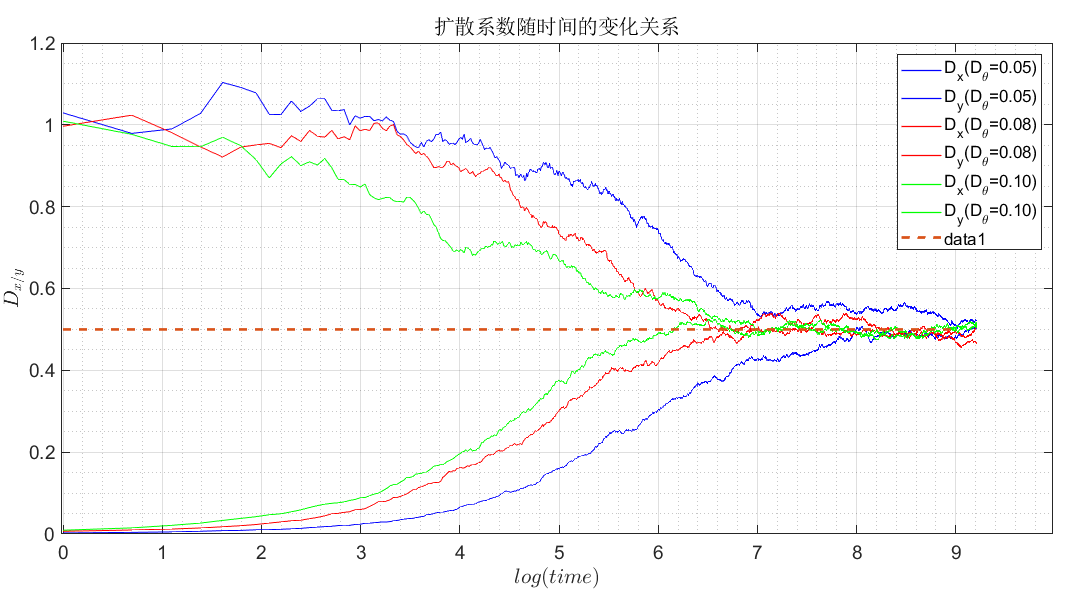
\includegraphics[width=6in]{D}
		\caption{不同$D_t$下数值计算结果(图中的$D_\theta$即为$D_t$)}
	\end{figure}

	\begin{flushleft}
		
		图中虚线为$D=0.5001$。从图上可以明显看出,$x,y$方向上的扩散一开始差别非常大,这是因为我设定了初始$\theta_0=0$,一开始沿着$x$方向阻力很小,很容易扩散,所以体现出$D_x\approx D_1^2=1>D_y\approx D_2^2=10^{-4}$。但是由于$D_x,D_y$并非是完全解耦的,它们通过“随机游走”的$\theta$联系起来,最后应当变得各向同性,体现就在:
		$D_x=D_y=\frac{1}{2}(D_1^2+D_2^2)\approx0.5001$。同时,可以看出随着$D_t$增大,达到各向同性的时间减小,这也符合物理直观。
	\end{flushleft}


	\subsection{四阶累计量的特征}
	
	如前所述,为了和标准无$\theta$耦合的情形对比,采用10000个系统统计四阶累计量。
	
	\begin{figure}[H]
		\centering  %图片全局居中
		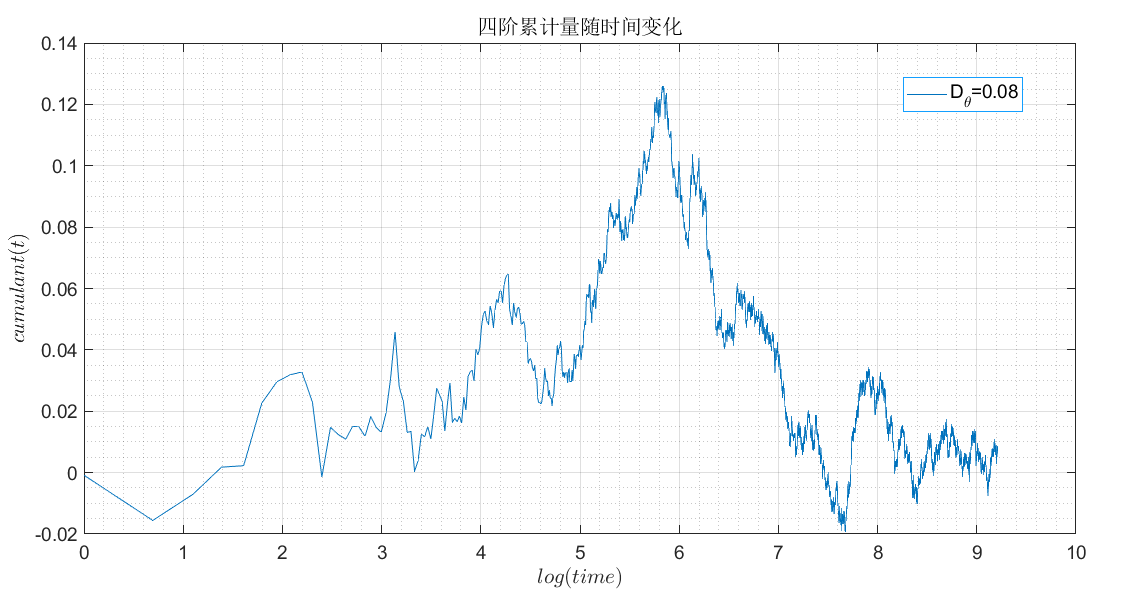
\includegraphics[width=6in]{cumulant}
		\caption{$D_t=0.08$下数值计算结果(图中的$D_\theta$即为$D_t$)}
	\end{figure}

	\begin{flushleft}
		四阶统计量体现出峰状的结构。从物理图像上来讲,一开始$\theta$各向同性的平均作用不明显,尚可认为$x,y$解耦,因而统计量较小,和正态分布体现出相同特征。最后由于$x,y$扩散也已稳定,它们等价,也呈现出正态的特点。唯有在中间尚未达到各向同性时呈现出峰状的最大偏离特征。为了进一步得到平滑曲线,可以进一步增大系统数量,以期达到更好的效果。不过这里体现出的基本特征已经和参考文献[1]中的非常相似了。
	\end{flushleft}
%\begin{figure}[H]
%	\centering  %图片全局居中
%	\subfigure[N=2]{
%		
%		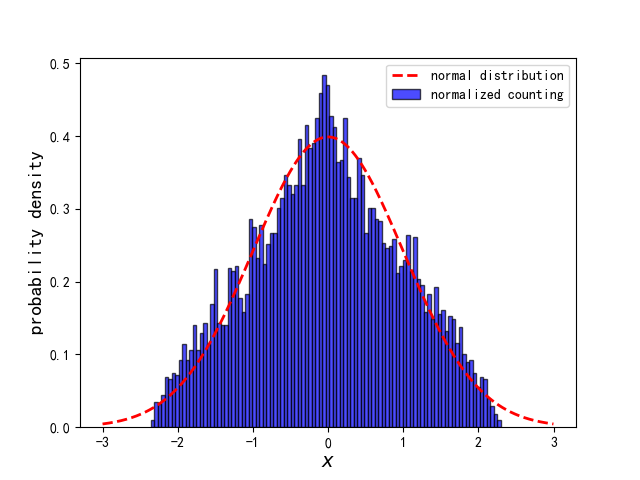
\includegraphics[width=0.45\textwidth]{../result/self_2.png}}
%	\subfigure[N=5]{
%		
%		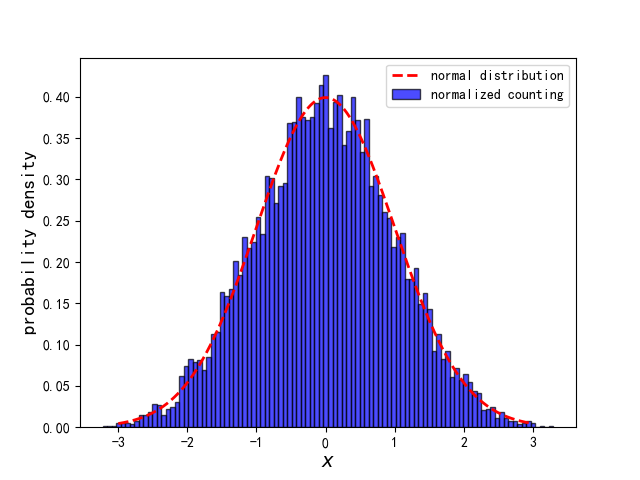
\includegraphics[width=0.45\textwidth]{../result/self_5.png}}
%	
%	\subfigure[N=10]{
%		
%		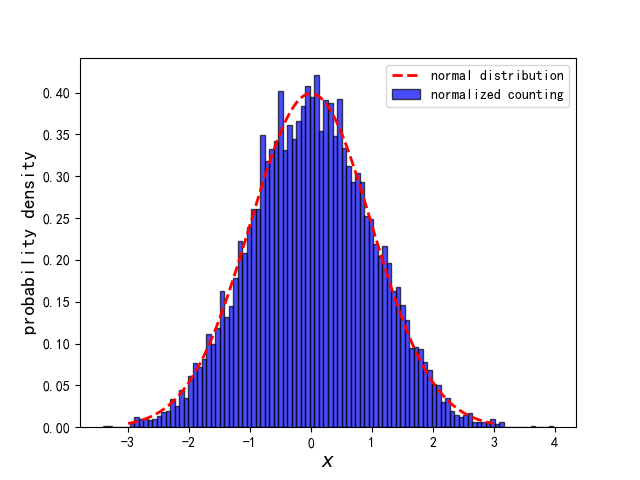
\includegraphics[width=0.45\textwidth]{../result/self_10.png}}
%	\subfigure[N=1000]{
%		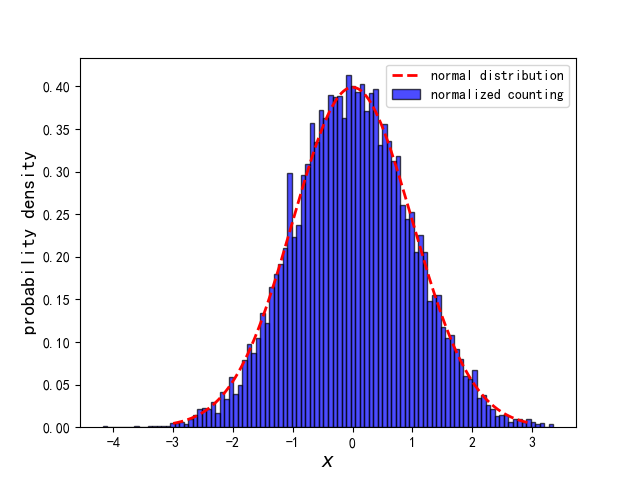
\includegraphics[width=0.45\textwidth]{../result/self_1000.png}}
%		
%	\caption{不同$N$下面的$Y$分布情况}
%\end{figure}


%		\begin{figure}[H]
%		\centering  %图片全局居中
%		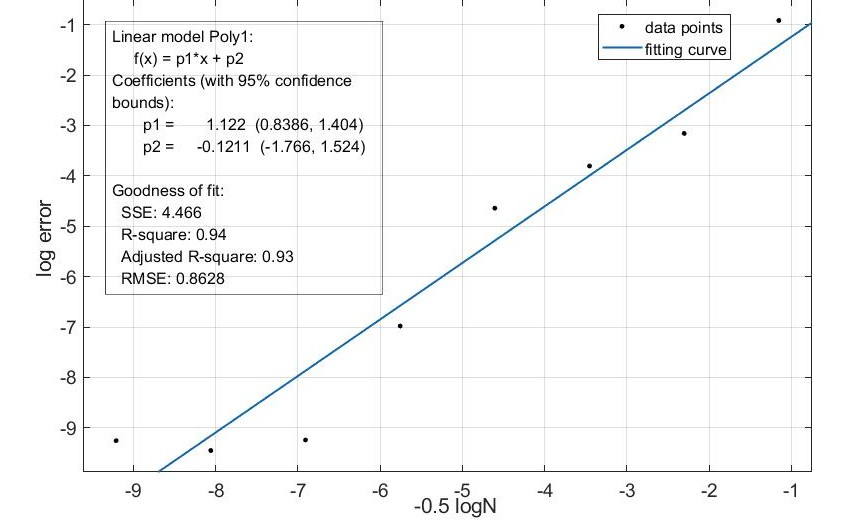
\includegraphics[width=6in]{../figure/single.jpg}
%		\caption{$log(\epsilon)-log(\frac{1}{\sqrt{N}})$}
%	\end{figure}
	

%	\begin{figure}[H]
%		\centering  %图片全局居中
%		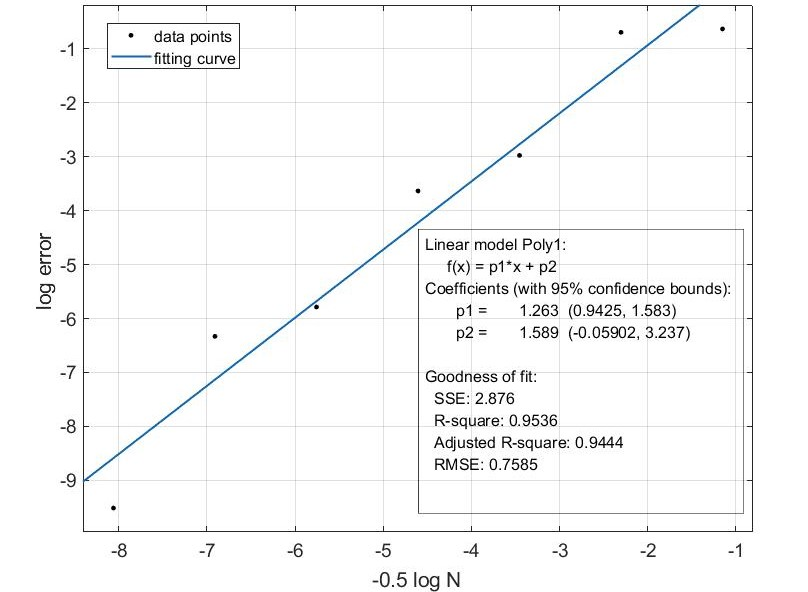
\includegraphics[width=6in]{../figure/multi.jpg}
%		\caption{$log(\epsilon)-log(\frac{1}{\sqrt{N}})$}
%	\end{figure}

	\newpage
	\section{总结}
	\begin{itemize}
		\item 本次实验通过建立最简单的模型模拟了带取向纳米棒的随机游走。进一步考虑修正模型也许得到多聚体随机游走模型[2]。
		\item 多出来的$\theta$自由度为$x,y$方向的随机游走提供了耦合,导致出一些与普通随机游走不同的有趣现象。
		\item 程序还需改进。有的地方动态分配多个大数组,明显减慢了运行速度。并且为了换不同的时间种子,用了几处$sleep$函数,也降低了运行速度。
	\end{itemize}
	
	
	
	\begin{thebibliography}{99}  
		\bibitem{ref1}Yilong Han, Ahmed M Alsayed, Maurizio Nobili, Jian Zhang, Tom C Lubensky, and Arjun G
		Yodh. Brownian motion of an ellipsoid. Science, 314(5799):626–630, 2006.
		\bibitem{ref2}Sethna J. Statistical mechanics: entropy, order parameters, and complexity[M]. Oxford University Press, 2006.
		\bibitem{ref3}中科大丁泽军计算物理讲义
	\end{thebibliography}
	
	
	
	
	\clearpage
\end{document}